% Autorska priprava k Realisticky.cz 020207; ulohy jsou autorske a obmenene.
% Zamerne nenahrazuje vyklad presnymi kopiemi cizich textu/prikladu.
\documentclass[11pt,a4paper]{article}
\input{../../sablony/pripravy/priprava.sty}
\usepackage{tikz}
\nastavPripravu{1. ročník}{Rovnice a nerovnice}{78}{Soustavy lineárních nerovnic}
\begin{document}
\blok{Návaznost a motivace}
Přípustný argument musí splnit několik podmínek současně. U soustavy proto hledáme průnik řešení jednotlivých nerovnic, nikoli jejich sjednocení.
\begin{definiceBox}
\textbf{Soustava nerovnic}. Soubor nerovnic se společnými neznámými; jeho řešením je množina všech hodnot, které vyhovují každé nerovnici zároveň.
\end{definiceBox}
\blok{Princip a odvození}
Každou nerovnici vyřeš samostatně, zobraz výslednou množinu na číselné ose a odečti jejich průnik. Naopak slovo „nebo“ obvykle vede k sjednocení. Hraniční bod zahrň jen tehdy, když jej splňují všechny podmínky.
\blok{Řešené příklady: od jednoduchého ke složitějšímu}
\begin{prikladReseniBox}[title={Příklad 1}]
Vyřešte soustavu $x>1$, $x\le4$.
\tcblower
\begin{align*}
K_1&=(1;+\infty) \\
 K_2&=(-\infty;4\rangle \\
 K_1\cap K_2&=(1;4\rangle
\end{align*}
\end{prikladReseniBox}
\begin{prikladReseniBox}[title={Příklad 2}]
Vyřešte $2x-3\ge1$, $x+2<7$.
\tcblower
\begin{align*}
2x-3&\ge1\Rightarrow x\ge2 \\
 x+2&<7\Rightarrow x<5 \\
 K&=\langle2;5)
\end{align*}
\end{prikladReseniBox}
\poznamka{Zpočátku vykresli dvě různá šrafování; barevné odlišování není nutné. Doporučuji první samostatnou úlohu zkontrolovat ještě před přechodem ke třetí.}
\blok{Grafický význam průniku na číselné ose}
Na \textbf{první} ose vyšrafujeme řešení první nerovnice, na \textbf{druhé} řešení druhé. \textbf{Společnou} část pak zakreslíme na třetí osu. Dvě podmínky současně znamenají \emph{průnik} množin; sjednocení odpovídá podmínce \uv{alespoň jedna}.
\begin{center}
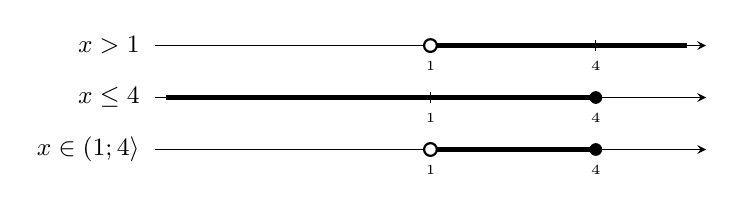
\begin{tikzpicture}[x=.7cm,y=.66cm,>=stealth]
\foreach \yy/\lbl in {2/{$x>1$},1/{$x\le4$},0/{$x\in(1;4\rangle$}}{
  \draw[->] (-4,\yy)--(6,\yy);
  \node[left] at (-4.1,\yy) {\small \lbl};
  \draw (1,\yy+.10)--(1,\yy-.10);
  \draw (4,\yy+.10)--(4,\yy-.10);
}
\draw[line width=2pt] (1,2)--(5.65,2);
\draw[fill=white,thick] (1,2) circle (2.3pt);
\draw[line width=2pt] (-3.8,1)--(4,1);
\fill (4,1) circle (2.3pt);
\draw[line width=2pt] (1,0)--(4,0);
\draw[fill=white,thick] (1,0) circle (2.3pt);
\fill (4,0) circle (2.3pt);
\foreach \yy in {0,1,2}{\node[below] at (1,\yy-.12) {\tiny $1$};\node[below] at (4,\yy-.12) {\tiny $4$};}
\end{tikzpicture}
\end{center}
\begin{zadaniReseniBox}[title={Kdy je průnik jen jediný bod?}]
Soustava $x\ge2$, $x\le2$.
\tcblower
\begin{align*}
K_1&=\langle2;+\infty),\\
K_2&=(-\infty;2\rangle,\\
K_1\cap K_2&=\{2\}.
\end{align*}
\end{zadaniReseniBox}

\blok{Samostatné procvičování}
\begin{zadaniReseniBox}[title={Úloha 1}]
Soustava $x\ge-2$, $x<3$, $x>0$.
\tcblower
\begin{align*}
K&=\langle-2;+\infty)\cap(-\infty;3)\cap(0;+\infty) \\
 K&=(0;3)
\end{align*}
\end{zadaniReseniBox}
\begin{zadaniReseniBox}[title={Úloha 2}]
Soustava $x\le-1$, $x\ge2$.
\tcblower
\begin{align*}
K&=(-\infty;-1\rangle\cap\langle2;+\infty) \\
 K&=\varnothing
\end{align*}
\end{zadaniReseniBox}
\begin{zadaniReseniBox}[title={Úloha 3}]
Soustava $3x+2\le11$, $2x-1>3$.
\tcblower
\begin{align*}
x&\le3\quad\text{a}\quad x>2 \\
 K&=(2;3\rangle
\end{align*}
\end{zadaniReseniBox}
\blok{Volitelná rezerva}
\begin{zadaniReseniBox}[title={Úloha 1}]
Určete $\{x\in\mathbb R\mid x\ge-1\;\text{a zároveň}\;x<2\}$.
\tcblower
\begin{align*}
K&=\langle-1;+\infty)\cap(-\infty;2) \\
 K&=\langle-1;2)
\end{align*}
\end{zadaniReseniBox}
\blok{Domácí úkol}
\begin{zadaniReseniBox}[title={Úloha 1}]
$3x-6\le0$ a současně $x>-1$.
\tcblower
\begin{align*}
x&\le2\quad\text{a}\quad x>-1 \\
 K&=(-1;2\rangle
\end{align*}
\end{zadaniReseniBox}
\begin{zadaniReseniBox}[title={Úloha 2}]
$2x+1>5$ a současně $x\le4$.
\tcblower
\begin{align*}
x&>2\quad\text{a}\quad x\le4 \\
 K&=(2;4\rangle
\end{align*}
\end{zadaniReseniBox}
\begin{zadaniReseniBox}[title={Úloha 3}]
$x<0$ a zároveň $x\ge0$.
\tcblower
\begin{align*}
K&=(-\infty;0)\cap\langle0;+\infty) \\
 K&=\varnothing
\end{align*}
\end{zadaniReseniBox}
\poznamka{Orientační časové rozvržení: 5 + 12 + 12 + 10 + 6 = 45 min. Přednost má pochopení jádra; rezerva není součástí časového součtu. Domácí úlohy jsou určeny na samostatnou práci, řešení zůstávají učiteli.}
\end{document}
